\documentclass[10pt]{beamer}
% \documentclass[handout,10pt]{beamer}
\usepackage{my_style}
%%%%%%%%%%%%%%%%%%%%%%%%%%%%%%%%%%%%%%%%%%%%%%%%%%%%%%%%%%%%%%%%%%%%%%%%
%%%%%%%%%%%%%%%%%%%%%%%%%%%%%%%%%%%%%%%%%%%%%%%%%%%%%%%%%%%%%%%%%%%%%%%%

\title[Math/CS 375]{Lecture 08 - A}
\subtitle{\S 8.4 Stationary Iterative Methods}

\begin{document}
% -------------------------------------------------
\begin{frame}
  \titlepage
\end{frame}
% -------------------------------------------------
\begin{frame}{Goals}
We will answer these questions:\\[3mm]
\begin{itemize}
    \item What is the main drawback of direct solvers? How do iterative solvers address this drawback? 
    \item What is Jacobi iteration?
    \item What is Gauss-Seidel?
    \item What is a fixed-point iteration and how is it related to Jacobi and GS?
\end{itemize}
\end{frame}


%%%%%%%%%%%%%%%%%%%%%%%%%%%%%%%%%%%%%%%%%%%%%%%%%%%%%%%%%%%%%%%%%%%%%
\sectionframe{Direct Solvers}
%%%%%%%%%%%%%%%%%%%%%%%%%%%%%%%%%%%%%%%%%%%%%%%%%%%%%%%%%%%%%%%%%%%%%

\begin{frame}{Direct Solvers}
\begin{itemize}

    \define{Direct Solver}{
    \textbf{Direct solvers} are a class of methods that find the exact solutions $x^*$ to the linear system $Ax=b$ (up to rounding error).
    }
    \bigskip
    \item We have been learning about direct solvers 
        \begin{itemize}
            \item Gaussian Elimination
            \item LU
            \item Cholesky Decomposition 
        \end{itemize}


    \bigskip 

    \item Why we like them: 
        \begin{itemize}
            \item Finds exact solution 
            \item Predictability 
            \item Great for smaller systems
            \item Don't need to worry about convergence
        \end{itemize}
    \bigskip 

    \item Matlab's backslash only uses direct solvers for dense $A$

\end{itemize}


\end{frame}
%%%%%%%%%%%%%%%%%%%%%%%%%%%%%%%%%%%%%%%%%%%
\begin{frame}{Complexity of Methods for Linear Systems}
Direct solvers

\begin{itemize}
\item diagonal solve: $\mO(n)$
\item tridiagonal solve: $\mO(n)$
\item triangular solve: $\mO(n^{2})$
\item $m$-band system: $\mO(m^{2}n)$
\vspace{3mm}

\item Gaussian Elimination with: $\mO(n^{3})$
\item partial pivoting adds $\mO(n^{2})$

\vspace{3mm}
\item LU/LDL/Cholesky factorization: $\mO(n^{3})$
\item one LU solve: $\mO(n^{2})$
\item solve $k$ different right-hand sides (with LU): $\mO(n^3 + k n^{2})$

\end{itemize}
\end{frame}

%%%%%%%%%%%%%%%%%%%%%%%%%%%%%%%%%%%%%%%%%%%
\begin{frame}{Complexity of Solvers}
\begin{center}
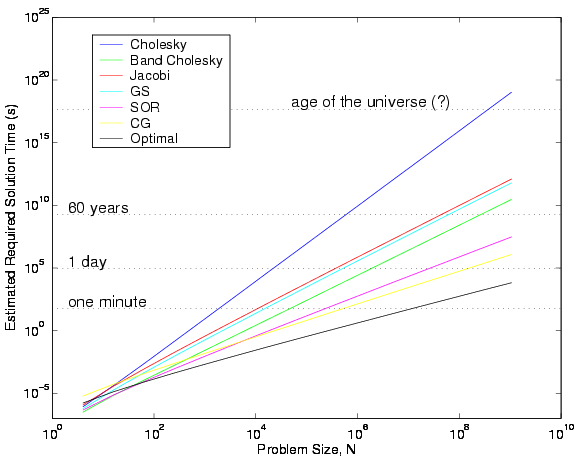
\includegraphics[scale=0.42]{figs/solvers.png}
\end{center}
\begin{itemize}
    \item log-log plot shows runtime versus size to solve an $N\times N$ system
    \item Direct solvers (even Cholesky) simply do not scale well for large $N$
\end{itemize}
\end{frame}
%%%%%%%%%%%%%%%%%%%%%%%%%%%%%%%%%%%%%%%%%%%
\begin{frame}{Complexity of Solvers}
\begin{center}
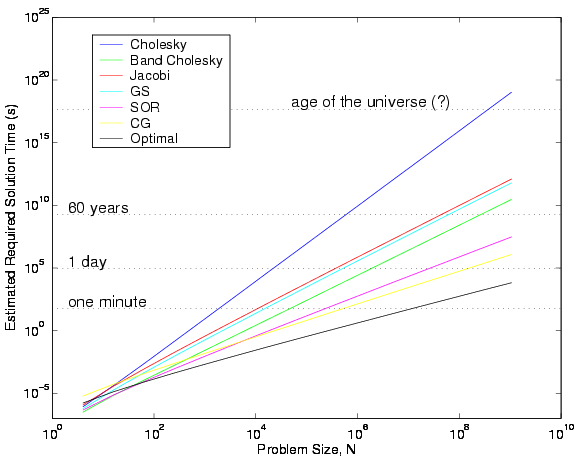
\includegraphics[scale=0.42]{figs/solvers.png}
\end{center}

\keyidea{For applications with a million unknowns, direct solvers are prohibitively slow.}

\end{frame}

%%%%%%%%%%%%%%%%%%%%%%%%%%%%%%%%%%%%%%%%%%%

\begin{frame}{Need for faster methods}
\begin{columns}
\begin{column}{0.45\textwidth}
\pgfimage[height=3cm]{./figs/pull1}

\begin{center}
  \begin{block}{}
    Accuracy
  \end{block}
\end{center}
\end{column}

\begin{column}{0.45\textwidth}
\pgfimage[height=3cm]{./figs/pull2}

\begin{center}
  \begin{block}{}
    Cost
  \end{block}
\end{center}
\end{column}
\end{columns}
\begin{itemize}
    \item Scalability is the biggest issue for direct solvers 
    \item Willing to trade exactness for speed
    \item<2> Use methods called \textbf{iterative solvers}
\end{itemize}
\end{frame}

%%%%%%%%%%%%%%%%%%%%%%%%%%%%%%%%%%%%%%%%%%%
\sectionframe{Iteratively Improve}
%%%%%%%%%%%%%%%%%%%%%%%%%%%%%%%%%%%%%%%%%%%

\begin{frame}{Iterative Methods}

\question{
If Gaussian elimination is taking too long and you stop
halfway, do you have an approximate solution?
\onslide<2->{
\\[2mm]
\textbf{Nothing}
}
}

\onslide<3->{
\define{Iterative Methods}{
\textbf{Iterative methods} construct a sequence of
approximate solutions
\[
    x^{(0)},\ x^{(1)},\ x^{(2)},\ldots
\]
starting from an initial guess $x^{(0)}$.
The integer $k$ is the \textbf{iteration index}.
}

\begin{itemize}
    \item Our goal is convergence to the true solution:
    \[
        x^{(k)} \longrightarrow x^*
        \qquad \text{as } k\to\infty.
    \]

    \item We can stop once the approximation is
    sufficiently accurate.

    \item For suitable problems, this can cost less
    than a direct solve.
\end{itemize}
}

\end{frame}

%%%%%%%%%%%%%%%%%%%%%%%%%%%%%%%%%%%%%%%%%%%

\begin{frame}{The Error}

\begin{itemize}
    \item Assume $A$ is nonsingular, and let $x^*$ be
    the exact solution of $Ax=b$.

    \item The error at iteration $k$ is
    \[
        e^{(k)} := x^* - x^{(k)}.
    \]

    \item Ideally, we would stop when
    \[
        \|e^{(k)}\| < \delta,
    \]
    where $\delta>0$ is a chosen error tolerance.

    \item \textbf{Issue:} We do not know $x^*$,
    so $e^{(k)}$ is unknown as well
\end{itemize}

\bigskip

\question{
How can we decide when to stop using quantities
we can actually compute?
}

\end{frame}

%%%%%%%%%%%%%%%%%%%%%%%%%%%%%%%%%%%%%%%%%%%

\begin{frame}{The Residual}{A Computable Measure}

\begin{itemize}
    \item \textbf{Idea}: use the residual instead
    \[
        r^{(k)} := b-Ax^{(k)}.
    \]

    \item It is related to the error by
    \[
        r^{(k)}
        = Ax^*-Ax^{(k)}
        = A e^{(k)}.
    \]
    \item Or solving for 
    $$
        e^{(k)}= A^{-1}r^{(k)}
    $$

    \item $r^{(k)}$ is not the same as $e^{(k)}$ - \textbf{Conditioning matters}
\end{itemize}

\keyidea{
We can compute the residual at every iteration and stop when
\[
    \|r^{(k)}\| = \|b-Ax^{(k)}\| < \delta,
\]
where $\delta>0$ is a chosen residual tolerance.
}
\end{frame}

%%%%%%%%%%%%%%%%%%%%%%%%%%%%%%%%%%%%%%%%%%%

\begin{frame}[fragile]{Typical Iterative Algorithm}

\begin{block}{Iterative Update}
  The update has the form
    \[
        \underbrace{x^{(k+1)}}_{\text{new}}
        =
        \underbrace{x^{(k)}}_{\text{old}}
        +
        \underbrace{c^{(k)}}_{\text{correction}}.
    \]
\end{block}

\begin{lstlisting}[mathescape]
r = b - A*x
for k = 1:kmax
    if norm(r) <= tol
        break
    end
    correction = compute_correction(A, r)
    x = x + correction
    r = b - A*x
end
\end{lstlisting}



\end{frame}

%%%%%%%%%%%%%%%%%%%%%%%%%%%%%%%%%%%%%%%%%%%

\begin{frame}{The Correction}{Part 1}

\question{
Suppose you start $x^{(0)}$. What is the ideal correction 
$$
x^{(1)} = x^{(0)}+c^{(0)}?
$$
}

\onslide<2->{

\begin{itemize}

    \item The ideal correction is $c^{(0)}=e^{(0)}$ because
    \begin{align*}
        x^{(1)} &= x^{(0)}+e^{(0)}\\
        &= x^{(0)}+x^*-x^{(0)}\\
        &= x^{*}
    \end{align*}

    \item Therefore, the best first step is 
    \begin{align*}
        x^{(1)} &= x^{(0)}+e^{(0)}\\
        &= x^{(0)}+A^{-1}r^{(0)}
    \end{align*}
\end{itemize}
}
\onslide<3>{
\question{Do you see a problem with this correction step?}
}

\end{frame}

%%%%%%%%%%%%%%%%%%%%%%%%%%%%%%%%%%%%%%%%%%%

\begin{frame}{The Correction}{Part 2}

\begin{itemize}
    \item \textbf{Problem}: the update 
    \[
        x^{(k+1)}=x^{(k)}+A^{-1}r^{(k)}.
    \]
    is nonsense because it requires $A^{-1}$
        \vfill 
    \item \textbf{Solution}: use an approximation of the inverse $Q^{-1}\approx A^{-1}s$
    \[
        x^{(k+1)}=x^{(k)}+Q^{-1}r^{(k)}.
    \]
\end{itemize}

\keyidea{
The strategy to iteratively improve the vector is
$$
x^{(k+1)}=x^{(k)}+Q^{-1}r^{(k)}
$$
where $Q\approx A$
}

\end{frame}

%%%%%%%%%%%%%%%%%%%%%%%%%%%%%%%%%%%%%%%%%%%

\begin{frame}{Stationary Iterative Solvers}

\define{Stationary Iteration}{
Choose $Q$ and initial guess $x^{(0)}$.
\begin{enumerate}
    \item Calculate $r^{(k)} = b-Ax^{(k)}$
    \item Solve $Qc^{(k)} = r^{(k)}$
    \item Update $x^{(k+1)} = x^{(k)}+c^{(k)}$
\end{enumerate}
The is called a \textbf{stationary iteration} because
the matrix $Q$ is fixed.
}

\begin{itemize}
    \item The choice of $Q$ determines the method.

    \item It affects both the cost per iteration
    and whether the iteration converges.
\end{itemize}

\question{
Which choices of $Q$ make the correction easy to compute?
}

\end{frame}

%%%%%%%%%%%%%%%%%%%%%%%%%%%%%%%%%%%%%%%%%%%
\sectionframe{Choices for $Q$}
%%%%%%%%%%%%%%%%%%%%%%%%%%%%%%%%%%%%%%%%%%%

\begin{frame}{A Simple Choice for $Q$}

\begin{itemize}
    \item \textbf{Idea:} Keep only the diagonal:
    \[
    A=
    \begin{bmatrix}
    2&-1&0\\
    -1&3&-1\\
    0&-1&2
    \end{bmatrix}
    \approx
    \begin{bmatrix}
    2&0&0\\
    0&3&0\\
    0&0&2
    \end{bmatrix}
    =Q=D.
    \]

    \item \textbf{Why?:} Inverse  $D^{-1}$ is cheap
    \[
    D^{-1}=
    \begin{bmatrix}
    1/2&0&0\\
    0&1/3&0\\
    0&0&1/2
    \end{bmatrix}.
    \]
\end{itemize}

\begin{block}{An Inexpensive Correction}
\[
    Dc^{(k)}=r^{(k)}
    \qquad\Longrightarrow\qquad
    c_i^{(k)}=\frac{r_i^{(k)}}{a_{ii}}.
\]
\end{block}

\end{frame}


%%%%%%%%%%%%%%%%%%%%%%%%%%%%%%%%%%%%%%%%%%%


\begin{frame}[fragile]{The Jacobi Iteration}

\begin{block}{Jacobi Update}
\[
    x^{(k+1)}=x^{(k)}+D^{-1}r^{(k)}.
\]
\end{block}

{
\method{Jacobi Iteration}
{System $Ax=b$, tolerance $\delta$}
{Approximate solution $\hat{x}$}
{Diagonal approximation $A\approx D$ to compute inexpensive corrections}
}

\begin{lstlisting}[mathescape]
$x = x^{(0)}$
for $k=1,\ldots,k_{\max}$
    $r = b-Ax$
    if $\|r\| \le \delta$, stop
    $c_i = r_i/a_{ii}$ for $i=1,\ldots,n$
    $x = x+c$
end
\end{lstlisting}


\end{frame}

%%%%%%%%%%%%%%%%%%%%%%%%%%%%%%%%%%%%%%%%%%%

\begin{frame}{Jacobi Example}{Part 1}

\begin{example}
Perform two Jacobi iterations to approximate the solution of \(Ax=b\):
\[
A=\begin{bmatrix}
\;2 & -1\\
-1 & \;2
\end{bmatrix},
\qquad
b=\begin{bmatrix}
1\\[2pt] 0
\end{bmatrix},
\qquad
x^{(0)}=\begin{bmatrix}
0\\[2pt] 0
\end{bmatrix}.
\]
\end{example}

\begin{itemize}
    \item First, construct $Q$ and $Q^{-1}$
\[
Q=D=\operatorname{diag}(A)=
\begin{bmatrix}
\;2 & 0\\
0 & \;2
\end{bmatrix}
\;\;\Longrightarrow\;\;
Q^{-1}=
\begin{bmatrix}
\;1/2 & 0\\
0 & \;1/2
\end{bmatrix}
\]
\item \textbf{Iteration 1}: compute $r^{(0)}$ and $x^{(1)}$
\[
r^{(0)} = b-Ax^{(0)} = b =
\begin{bmatrix}1\\ 0\end{bmatrix},\qquad
x^{(1)} = x^{(0)} + Q^{-1}r^{(0)} =
\begin{bmatrix}0\\ 0\end{bmatrix} +
\begin{bmatrix}\tfrac12\\ 0\end{bmatrix} =
\begin{bmatrix}\tfrac12\\ 0\end{bmatrix}.
\]
\end{itemize}

\end{frame}
%%%%%%%%%%%%%%%%%%%%%%%%%%%%%%%%%%%%%%%%%%%
\begin{frame}{Jacobi Example}{Part 2}

\begin{itemize}
    \item Compute the new residual:
    \[
    r^{(1)}
    =
    \begin{bmatrix}1\\0\end{bmatrix}
    -
    \begin{bmatrix}2&-1\\-1&2\end{bmatrix}
    \begin{bmatrix}1/2\\0\end{bmatrix}
    =
    \begin{bmatrix}0\\1/2\end{bmatrix}.
    \]

    \item Apply the correction:
    \[
    x^{(2)}
    =
    \begin{bmatrix}1/2\\0\end{bmatrix}
    +
    \begin{bmatrix}1/2&0\\0&1/2\end{bmatrix}
    \begin{bmatrix}0\\1/2\end{bmatrix}
    =
    \begin{bmatrix}1/2\\1/4\end{bmatrix}.
    \]
\end{itemize}

\begin{block}{How Close Are We?}
\[
    x^*=\begin{bmatrix}2/3\\1/3\end{bmatrix},
    \qquad
    \|x^{(2)}-x^*\|_2
    =\frac{\sqrt{5}}{12}
    \approx0.186.
\]
\end{block}

\end{frame}
%%%%%%%%%%%%%%%%%%%%%%%%%%%%%%%%%%%%%%%%%%%

\begin{frame}{Reduction in Normalized Residual}

\cols{
    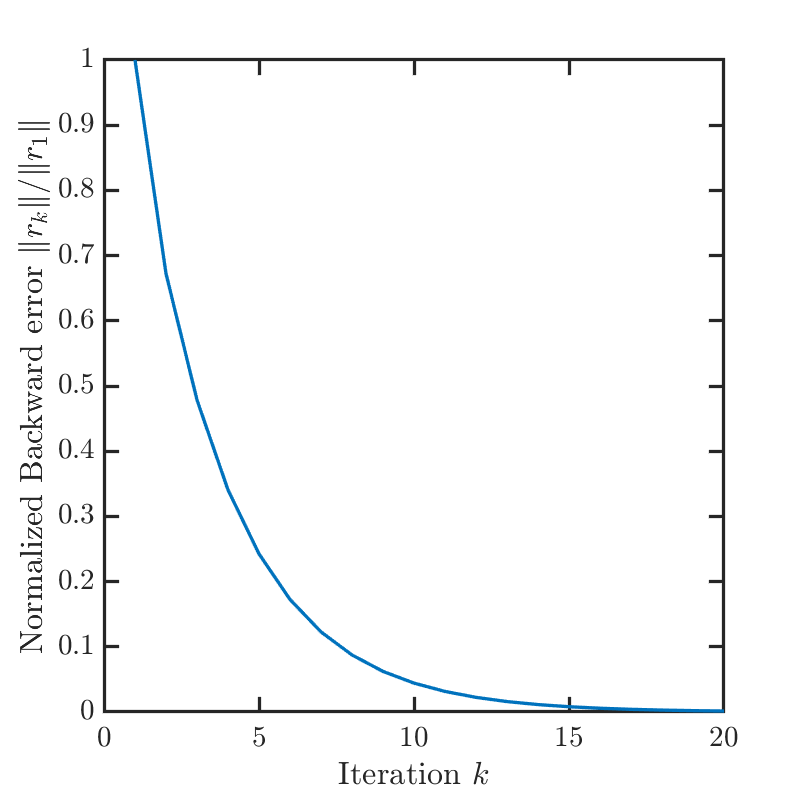
\includegraphics[scale=0.25]{figs/jacobi_res.png}
}{
    \begin{itemize}
        \item Track the \textbf{normalized residual}.
    \end{itemize}

    \begin{block}{Residual History}
    \[
        R_k=\frac{\|r^{(k)}\|}{\|r^{(1)}\|}.
    \]
    \end{block}

    \begin{itemize}
        \item Plot against iteration $k$.
        \item See \texttt{iterative\_methods.m}.
    \end{itemize}
}

\end{frame}

%%%%%%%%%%%%%%%%%%%%%%%%%%%%%%%%%%%%%%%%%%%

\begin{frame}{Matrix Splitting}
\begin{itemize}
    \item We can split up a square matrix like so
    $$
        \begin{bmatrix}\bullet & \bullet & \bullet & \bullet  \\
                    \bullet & \bullet & \bullet & \bullet \\
                    \bullet & \bullet & \bullet & \bullet \\
                    \bullet & \bullet & \bullet & \bullet \end{bmatrix} = 
            \begin{bmatrix}
                 &  &  &  \\
                \bullet &  &  &  \\
                \bullet & \bullet &  &  \\
                \bullet & \bullet & \bullet &  \end{bmatrix} +
            \begin{bmatrix}
                \bullet & &  & \\
                 & \bullet & &  \\
                 &  & \bullet &  \\
                 &  &  & \bullet \end{bmatrix} + 
            \begin{bmatrix}
                 & \bullet & \bullet & \bullet \\
                 &  & \bullet & \bullet \\
                 &  &  & \bullet \\
                 &  &  &  \end{bmatrix}        
    $$
    \bigskip
    \item Let $A = D  + C_U +  C_L$, where $C_U$ and $C_L$ are the strictly upper and lower triangular components of $A$, respectively.
    \bigskip
\end{itemize}
\end{frame}

%%%%%%%%%%%%%%%%%%%%%%%%%%%%%%%%%%%%%%%%%%%

\begin{frame}{Example of Matrix Splitting}

\begin{example}
Split the following matrix
\[
A =
\begin{bmatrix}
4 & -1 & 0 & 0 \\
-1 & 4 & -1 & 0 \\
0 & -1 & 4 & -1 \\
0 & 0 & -1 & 3
\end{bmatrix}
\]
\end{example}
We split it into three parts:
\[
A = D + C_L + C_U
\]
where:
\[
D = \begin{bmatrix}
4 & 0 & 0 & 0 \\
0 & 4 & 0 & 0 \\
0 & 0 & 4 & 0 \\
0 & 0 & 0 & 3
\end{bmatrix}, \quad
C_L = \begin{bmatrix}
0 & 0 & 0 & 0 \\
-1 & 0 & 0 & 0 \\
0 & -1 & 0 & 0 \\
0 & 0 & -1 & 0
\end{bmatrix}, \quad
C_U = \begin{bmatrix}
0 & -1 & 0 & 0 \\
0 & 0 & -1 & 0 \\
0 & 0 & 0 & -1 \\
0 & 0 & 0 & 0
\end{bmatrix}.
\]
\end{frame}

%%%%%%%%%%%%%%%%%%%%%%%%%%%%%%%%%%%%%%%%%%%
\begin{frame}[fragile,shrink]{Splitting in Matlab}

\begin{lstlisting}[mathescape]
>> A = ones(4,4)  
     1     1     1     1
     1     1     1     1
     1     1     1     1
     1     1     1     1

>> tril(A) % lower triangular 
     1     0     0     0
     1     1     0     0
     1     1     1     0
     1     1     1     1

>> triu(A) % upper triangular 
     1     1     1     1
     0     1     1     1
     0     0     1     1
     0     0     0     1

>> tril(A,-1) % lower triangular without the diagonal
     0     0     0     0
     1     0     0     0
     1     1     0     0
     1     1     1     0
\end{lstlisting}

\end{frame}

%%%%%%%%%%%%%%%%%%%%%%%%%%%%%%%%%%%%%%%%%%%

\begin{frame}{Matrix Splitting Approximations}


 \begin{block}{Diagonal Only}
     This approximation $A\approx Q = D$ yields \textbf{Jacobi iteration} 
    $$
        \begin{bmatrix}\bullet & \bullet & \bullet & \bullet  \\
                    \bullet & \bullet & \bullet & \bullet \\
                    \bullet & \bullet & \bullet & \bullet \\
                    \bullet & \bullet & \bullet & \bullet \end{bmatrix} \approx 
            \begin{bmatrix}
                \bullet & &  & \\
                 & \bullet & &  \\
                 &  & \bullet &  \\
                 &  &  & \bullet \end{bmatrix} 
    $$
 \end{block}

    \begin{block}{Diagonal + Lower}
        
  This approximation $A\approx Q = D+C_L$ leads to \textbf{Gauss-Seidel iteration}
        $$
        \begin{bmatrix}\bullet & \bullet & \bullet & \bullet  \\
                    \bullet & \bullet & \bullet & \bullet \\
                    \bullet & \bullet & \bullet & \bullet \\
                    \bullet & \bullet & \bullet & \bullet \end{bmatrix} \approx 
            \begin{bmatrix}
                 &  &  &  \\
                \bullet &  &  &  \\
                \bullet & \bullet &  &  \\
                \bullet & \bullet & \bullet &  \end{bmatrix} +
            \begin{bmatrix}
                \bullet & &  & \\
                 & \bullet & &  \\
                 &  & \bullet &  \\
                 &  &  & \bullet \end{bmatrix} 
    $$
    \end{block}

\end{frame}

%%%%%%%%%%%%%%%%%%%%%%%%%%%%%%%%%%%%%%%%%%%

\begin{frame}[fragile]{Gauss-Seidel (GS)}
\begin{itemize}
    \item Approximate $A$ with $Q =\mathrm{tril}(A)$
    \item In Matlab, \texttt{tril(A,-1)} returns the lower portion of matrix $A$
    \item Then the algorithm is 
\begin{lstlisting}[mathescape]
$x = x^{(0)}$
$Q = D + C_L$ 
for $k=1$ to $k_{max}$
    $r = b - Ax$
    if $\|r\| \leq tol$, stop
    $x= x + Q^{-1} r$
end
\end{lstlisting}
\end{itemize}
\vspace{0.1in}
\method{Gauss-Seidel}
{Given system $Ax=b$, tolerance $\epsilon$}
{Approximate solution $\hat{x}$}
{GS has a better approximation to $A^{-1}$ than Jacobi. $Q^{-1}$ can be computed relatively quickly because it is triangular.}
\end{frame}

%%%%%%%%%%%%%
\begin{frame}{Key Difference}

\begin{itemize}
    \item Same system and initial guess:
    \[
        A=\begin{bmatrix}2&-1\\-1&2\end{bmatrix},
        \qquad
        b=\begin{bmatrix}1\\0\end{bmatrix},
        \qquad
        x^{(0)}=\begin{bmatrix}0\\0\end{bmatrix}.
    \]
    \item First residual: $r^{(0)}=b$.
\end{itemize}

\begin{block}{Jacobi: Diagonal Solve}
\[
    \begin{bmatrix}2&0\\0&2\end{bmatrix}
    \begin{bmatrix}c_1\\c_2\end{bmatrix}
    =
    \begin{bmatrix}1\\0\end{bmatrix}
    \quad\Longrightarrow\quad
    c_1=\frac12,\qquad c_2=0.
\]
\end{block}

\begin{block}{Gauss-Seidel: Forward Substitution}
\[
    \begin{bmatrix}2&0\\-1&2\end{bmatrix}
    \begin{bmatrix}c_1\\c_2\end{bmatrix}
    =
    \begin{bmatrix}1\\0\end{bmatrix}
    \quad\Longrightarrow\quad
    c_1=\frac12,\qquad c_2=\frac{c_1}{2}=\frac14.
\]
\end{block}

\begin{itemize}
    \item Update $x^{(1)}=x^{(0)}+c$:
    \[
        x_{\mathrm{Jacobi}}^{(1)}
        =\begin{bmatrix}1/2\\0\end{bmatrix},
        \qquad
        x_{\mathrm{GS}}^{(1)}
        =\begin{bmatrix}1/2\\1/4\end{bmatrix}.
    \]
\end{itemize}

\end{frame}
% %%%%%%%%%%%%%%%%%%%%%%%%%%%%%%%%%%%%%%%%%%%
\begin{frame}{Actual Performance}

\begin{figure}
    \centering
    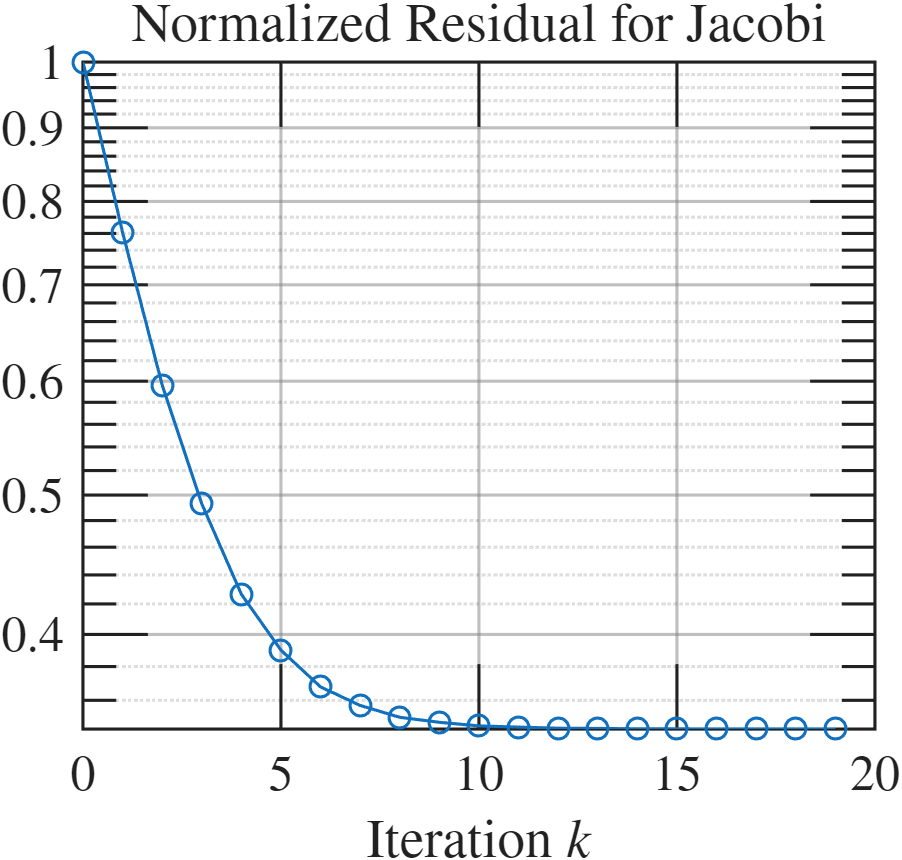
\includegraphics[width=0.45\linewidth]{figs/jac.png}
    \onslide<2>{
    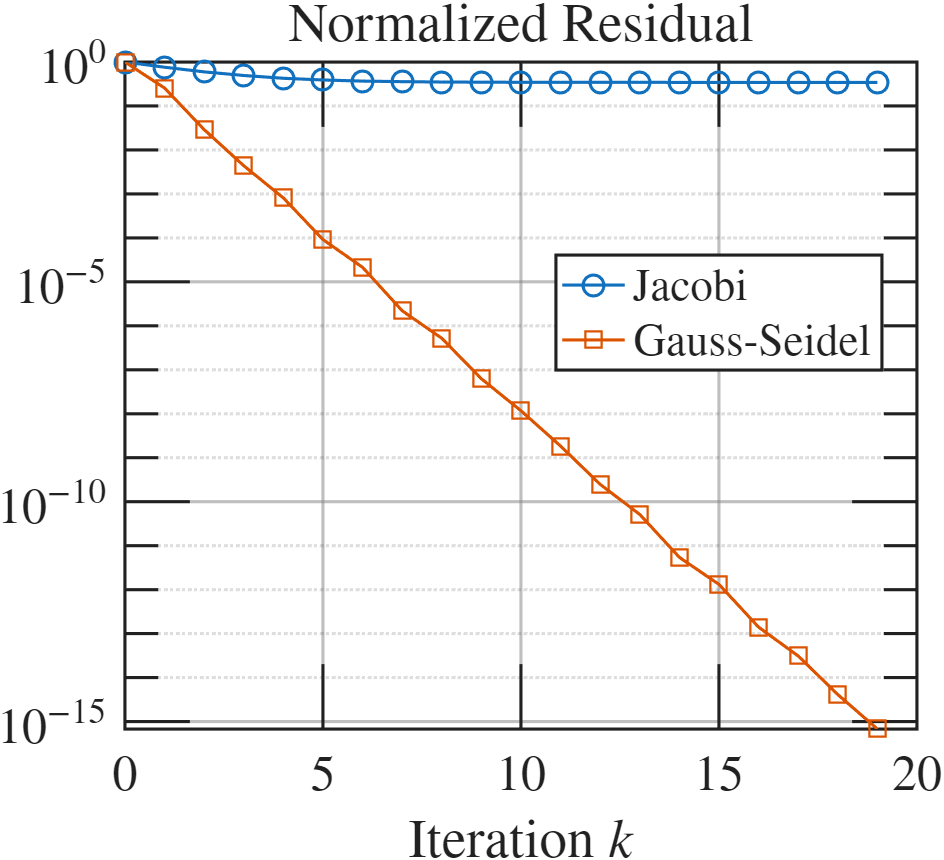
\includegraphics[width=0.45\linewidth]{figs/gs_jac.png}
    }
    \caption{Numerical results for solving $Ax=b$ with Jacobi and GS}
\end{figure}
    
\end{frame}


% \begin{frame}{Component-Wise Updates}

% \begin{itemize}
%     \item Solve row $i$ of $Ax=b$ for $x_i$:
%     \[
%         x_i=\frac{1}{a_{ii}}
%         \left(b_i-\sum_{j\ne i}a_{ij}x_j\right).
%     \]
% \end{itemize}

% \begin{block}{Jacobi: Use the Previous Iterate}
% \[
%     x_i^{(k+1)}
%     =
%     \frac{1}{a_{ii}}
%     \left(b_i-\sum_{j\ne i}a_{ij}x_j^{(k)}\right).
% \]
% \end{block}

% \begin{block}{Gauss-Seidel: Use New Values Immediately}
% \[
%     x_i^{(k+1)}
%     =
%     \frac{1}{a_{ii}}
%     \left(
%     b_i
%     -\sum_{j=1}^{i-1}a_{ij}x_j^{(k+1)}
%     -\sum_{j=i+1}^{n}a_{ij}x_j^{(k)}
%     \right).
% \]
% \end{block}

% \end{frame}

% %%%%%%%%%%%%%%%%%%%%%%%%%%%%%%%%%%%%%%%%%%%
% \begin{frame}{Gauss-Seidel Example}

% \begin{example}
% Use the same system and initial guess:
% \[
%     \begin{cases}
%         2x_1-x_2=1,\\
%         -x_1+2x_2=0,
%     \end{cases}
%     \qquad
%     x^{(0)}=\begin{bmatrix}0\\0\end{bmatrix}.
% \]
% \end{example}

% \begin{block}{Update in Order}
% \[
%     x_1^{(k+1)}=\frac{1+x_2^{(k)}}{2},
%     \qquad
%     x_2^{(k+1)}=\frac{x_1^{(k+1)}}{2}.
% \]
% \end{block}

% \begin{itemize}
%     \item First iteration:
%     \[
%         x_1^{(1)}=\frac{1+0}{2}=\frac12,
%         \qquad
%         x_2^{(1)}=\frac{1/2}{2}=\frac14.
%     \]

%     \item Second iteration:
%     \[
%         x_1^{(2)}=\frac{1+1/4}{2}=\frac58,
%         \qquad
%         x_2^{(2)}=\frac{5/8}{2}=\frac{5}{16}.
%     \]
% \end{itemize}

% \end{frame}

% %%%%%%%%%%%%%%%%%%%%%%%%%%%%%%%%%%%%%%%%%%%
% \begin{frame}{Jacobi vs. Gauss-Seidel}

% \begin{itemize}
%     \item Same system, same initial guess:
% \end{itemize}

% \[
% \begin{array}{c|c|c}
%     k & \text{Jacobi} & \text{Gauss-Seidel}\\ \hline
%     0 &
%     \begin{bmatrix}0\\0\end{bmatrix} &
%     \begin{bmatrix}0\\0\end{bmatrix}\\[4mm]
%     1 &
%     \begin{bmatrix}1/2\\0\end{bmatrix} &
%     \begin{bmatrix}1/2\\1/4\end{bmatrix}\\[4mm]
%     2 &
%     \begin{bmatrix}1/2\\1/4\end{bmatrix} &
%     \begin{bmatrix}5/8\\5/16\end{bmatrix}
% \end{array}
% \]

% \begin{block}{Exact Solution}
% \[
%     x^*=\begin{bmatrix}2/3\\1/3\end{bmatrix}.
% \]
% \end{block}

% \begin{itemize}
%     \item Gauss-Seidel makes more progress per iteration
%     \textbf{in this example}.
% \end{itemize}

% \end{frame}



%%%%%%%%%%%%%%%%%%%%%%%%%%%%%%%%%%%%%%%%%%%\
\sectionframe{Fixed-Point Iteration}
%%%%%%%%%%%%%%%%%%%%%%%%%%%%%%%%%%%%%%%%%%%
\begin{frame}{Old Calculator}
\cols{
    \begin{figure}
        \centering
        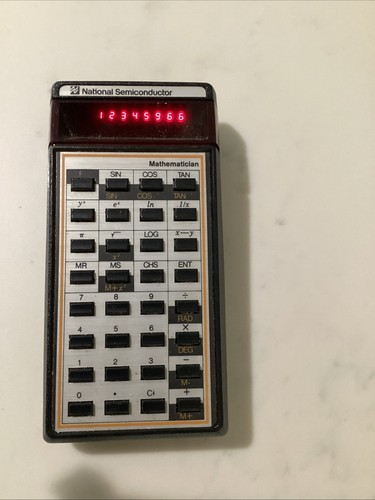
\includegraphics[width=0.95\linewidth]{figs/s-l500.jpg}
    \end{figure}
}{
\begin{itemize}
    \item Old calculators had a cosine button
    \item It calculates the cosine of whatever number is on screen
    \item If keep you mashing cosine you eventually get... 
     $$
    0.739085133215$$
\end{itemize}

}

\end{frame}


\begin{frame}{Fixed-Point Iteration}

    \begin{block}{Problem}
        Suppose your goal is to solve 
        $$x-\cos x=0$$
    \end{block}
    
    Here is one way:
    \begin{itemize}
        \item Rearrange the equation 
            \begin{align*}
                x&-\cos x= 0\\
                x&= \cos x
            \end{align*}
        \item Turn the equation into an iteration
        $$
        x = \cos x \quad\longrightarrow \quad x_{n+1} = \cos (x_n)
        $$
        \item Choose an initial guess and iterate 
            $$x_{n+1} = \cos(x_n)$$
            for $n = 1, 2, 3, \ldots$
    \end{itemize}
\end{frame}

\begin{frame}{Example Calculation}
    \begin{enumerate}
        \item Start with \( x_0 = 0 \)
        \item Calculate:
        \begin{align*}
            x_1 &= \cos(0) = 1 \\
            x_2 &= \cos(1) \approx 0.5403 \\
            x_3 &= \cos(0.5403) \approx 0.8576 \\
            x_4 &= \cos(0.8576) \approx 0.6543 \\
            & \vdots
        \end{align*}
        \item Continue until convergence (approximately \( x \approx 0.739 \)).
    \end{enumerate}
    \method{Fixed Point Iteration}{Function $f(x)$, starting guess $x_0$, tolerance $\epsilon$}{Approximate root of $f(x)$}{A simple method that transforms an equation into an iteration.}
\end{frame}


\begin{frame}{How it Works}{Transform equation into iteration}
    
    \begin{block}{The Equation to Solve}
        $$x = g(x)$$
    \end{block}
\begin{center} 
$\downarrow$ 
\end{center} \vspace{-2mm}
\begin{block}{Iteration}
\begin{equation*}
    x_{n+1} = g(x_{n})
\end{equation*}
\end{block}
\begin{center} 
$\downarrow$ 
\end{center}\vspace{-2mm}
\begin{block}{The Method}
\begin{enumerate}
    \item Choose starting guess $x_0$
    \item Iterate $x_{n+1} = g(x_n)$
    \item Repeat until $|x_{n+1} - x_n| < \delta$
\end{enumerate}
\end{block}
\end{frame}

%%%%%%%%%%%%%

\begin{frame}{Why Fixed-point Iteration?}
\begin{itemize}
    \item Fixed-point iteration is one of the simplest ways to solve equations iteratively.\\[5mm] 
    
    \item Just as we rewrite $f(x)=0$ as $x=g(x)$ to iterate scalar functions, we can rewrite the linear equation $Ax=b$ to iteratively.\\[5mm] 
\end{itemize}

\begin{block}{Key Idea}
    Jacobi and GS are actually just fixed-point iterations with matrices and vectors.    
\end{block}
\end{frame}

%%%%%%%%%%%%%%%%%%

\begin{frame}{Alternate Derivation of Jacobi}
    \begin{itemize}
        \item Split up the $A$ matrix like so $A = D +C_L + C_U$
            \vspace{3mm}
        \item Then $Ax=b$ becomes $(D +C_L + C_U)x = b$
            \vspace{3mm}
        \item We can rewrite that as 
            \begin{align*}
                (D +C_L + C_U)x &= b\\
                Dx &=   -(C_L + C_U)x + b\\
                x &=   -D^{-1}(C_L + C_U)x + D^{-1}b
            \end{align*}
        \item Treat it as a fixed-point iteration and we get \textbf{Jacobi Iteration} 
            $$ x^{(k+1)} =  -D^{-1}(C_L + C_U)x^{(k)} + D^{-1}b$$
    \end{itemize}
\end{frame}

%%%%%%%%%%%%%%%%%%%

\begin{frame}{Alternate Derivation of Jacobi}
    \begin{block}{The Equation to Solve}
        $$Ax = b$$
    \end{block}
\begin{center} 
$\updownarrow$ same 
\end{center} \vspace{-2mm}
\begin{block}{Equation with Matrix Splitting}
\[
    x=-D^{-1}(C_L+C_U)x+D^{-1}b.
\]
\end{block}
\begin{center} 
$\downarrow$ 
\end{center}\vspace{-2mm}
\begin{block}{Jacobi Iteration}
$$ x^{(k+1)} =   -D^{-1}(C_L + C_U)x^{(k)} + D^{-1}b$$
\end{block}
\end{frame}

% \begin{frame}{Equivalent Forms of Jacobi}
% \begin{block}{Residual Form}
%     $$\begin{cases}
%     r^{(k)} = b - Ax^{(k)} \\
%     x^{(k+1)} = x^{(k)} + D^{-1} r^{(k)}
%     \end{cases}$$
% \end{block}
% \begin{block}{Rearranged System}
%     \begin{align*}
% 	D x^{(k)} &= (D-A) x^{(k-1)} + b\\
% \end{align*}
% \end{block}
% \begin{block}{Fixed-point Form}
%         \begin{align*}
% 	x^{(k)} &= -D^{-1}(C_L + C_U) x^{(k-1)} + D^{-1}b\\
% \end{align*}
% \end{block}
% \end{frame}

\begin{frame}{Jacobi as a Fixed-Point Iteration}

\begin{itemize}
    \item Start with our example:
    \[
        \begin{cases}
            2x_1-x_2=1,\\
            -x_1+2x_2=0.
        \end{cases}
    \]

    \item Solve each equation for its diagonal variable:
    \[
        x_1=\frac{1+x_2}{2},
        \qquad
        x_2=\frac{x_1}{2}.
    \]
\end{itemize}

\begin{block}{Turn the Equations into an Iteration}
\[
    \boxed{x_1^{(k+1)}=\frac{1+x_2^{(k)}}{2}},
    \qquad
    \boxed{x_2^{(k+1)}=\frac{x_1^{(k)}}{2}}.
\]
\end{block}

% \begin{itemize}
%     \item Starting from $(x_1^{(0)},x_2^{(0)})=(0,0)$:
%     \[
%         (0,0)
%         \longrightarrow
%         \left(\frac12,0\right)
%         \longrightarrow
%         \left(\frac12,\frac14\right).
%     \]
% \end{itemize}

\keyidea{
This is Jacobi in component form:
use the \textbf{old values} in both equations.
}

\end{frame}

\begin{frame}[shrink]{Jacobi Example (Again)}

\begin{example}
Perform two Jacobi iterations starting from
$x^{(0)}=(0,0)^T$:
\[
    \begin{cases}
        2x_1-x_2=1,\\
        -x_1+2x_2=0.
    \end{cases}
\]
\end{example}

\begin{block}{Fixed-Point Formulas}
\[
    x_1^{(k+1)}=\frac{1+x_2^{(k)}}{2},
    \qquad
    x_2^{(k+1)}=\frac{x_1^{(k)}}{2}.
\]
\end{block}

\begin{itemize}
    \item \textbf{Iteration 1:} Use $(x_1^{(0)},x_2^{(0)})=(0,0)$.
    \[
        x_1^{(1)}=\frac{1+0}{2}=\frac12,
        \qquad
        x_2^{(1)}=\frac{0}{2}=0.
    \]

    \item \textbf{Iteration 2:} Use $(x_1^{(1)},x_2^{(1)})=(1/2,0)$.
    \[
        x_1^{(2)}=\frac{1+0}{2}=\frac12,
        \qquad
        x_2^{(2)}=\frac{1/2}{2}=\frac14.
    \]
\end{itemize}
\end{frame}

%%%%%%%%%%%%%%%%%%%%%%%%%%%%%%%%%%%%%%%%%%%


\sectionframe{Moving Forward}

\begin{frame}{Summary}
    \begin{itemize}
    \item For large systems, factorization can be expensive in both time and memory.
        \vfill 
        \item Stationary solvers improve upon an approximate solution 
        $$\begin{cases}
    r^{(k)} = b - Ax^{(k)} \\
    x^{(k+1)} = x^{(k)} + Q^{-1} r^{(k)}
    \end{cases}$$
        \item Choosing $Q=D$ (diagonal) gives you the Jacobi iteration
        \vfill
        \item Choosing $Q=D+C_L$ (diagonal + lower) gives you Gauss-Seidel.
    \end{itemize}
\end{frame}

\begin{frame}{Moving Forward}
    \begin{itemize}
        \item Does the Jacobi iteration always converge?
        \vfill 
        \item What is the best way to implement stationary solvers?
        \vfill 
        \item What are sparse matrices? 
        \vfill 
        \item How do sparse matrices work with stationary solvers?
        \vfill 
    \end{itemize}
\end{frame}

\end{document}